\documentclass[]{standalone}
\usepackage{tikz}
\begin{document}
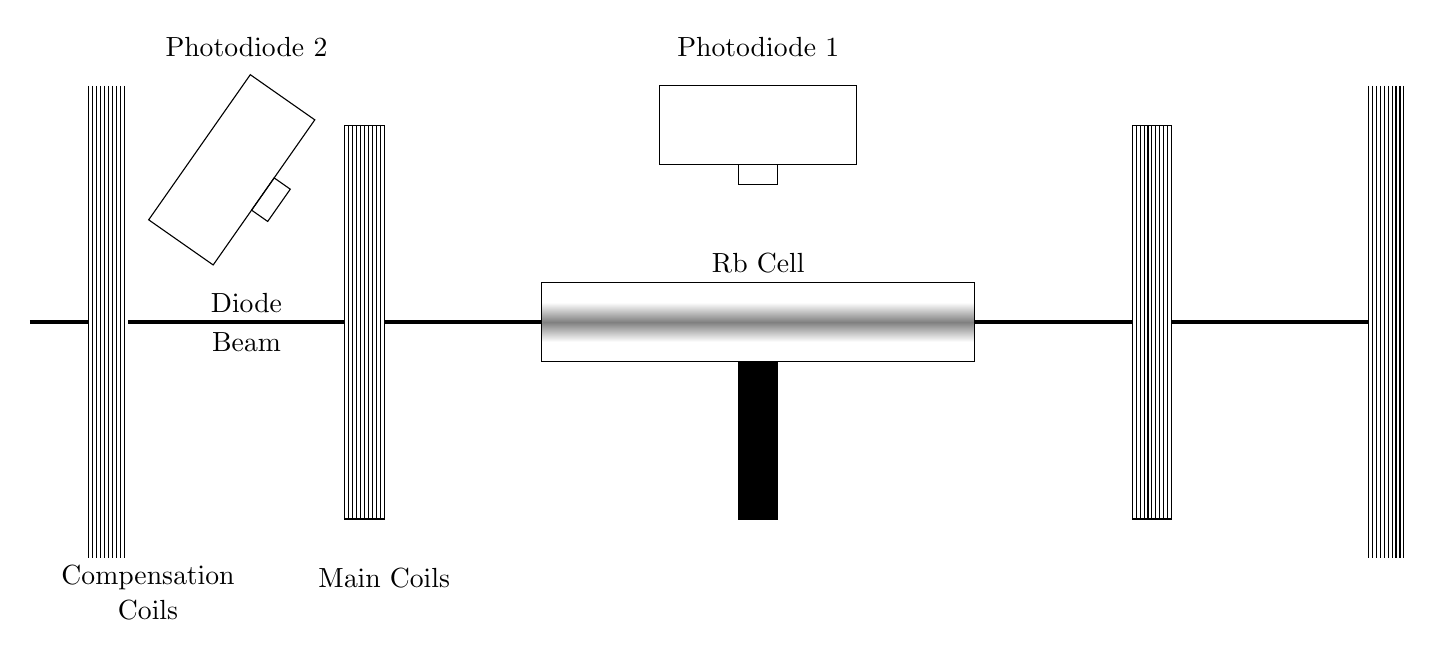
\begin{tikzpicture}
		\draw  (0,2.5) rectangle (.5,-2.5);
		\draw  (10,2.5) rectangle (10.5,-2.5);
		\node at (-1.25,.25) {Diode};
		\node at (-1.25,-.25) {Beam};
		%\draw[line width = 2.0pt] (-2,-.75) rectangle (-.5,.75);
		%main coils
	\foreach \index in {0,0.05,0.1,...,.5}
		{
			\draw (\index,2.5) -- (\index, -2.5);
			\draw (\index +10,2.5) -- (\index+10, -2.5);
		}
		%compensation coils
	\foreach \index in {0,0.05,0.1,...,.5}
		{
			\draw (\index,3.0)+(-3.25,0) -- +(-3.25,-6);
			\draw (\index+10,3.0)+(3,0) -- +(3,-6);
		}
	\draw[fill = black] (5.0,-2.5) rectangle (5.5,-.5);
	\draw (2.5,-.5) rectangle (8,.5) node at (5.25,.75) {Rb Cell};
	\draw[line width = 1.6pt] (-.5,0) -- (0,0);
	\draw[line width = 1.6pt] (.5,0) -- (2.5,0);
	\draw[line width = 1.6pt] (-4.0,0) -- (-3.25,0);
	\draw[line width = 1.6pt] (-2.75,0) -- (-.5,0);
	%\draw[line width = 3.6pt] (2.5,0) -- (8,0);
	\shade[bottom color = white, top color = gray] (2.51,0) rectangle (7.99,-.25);
	\shade[top color = white, bottom color = gray] (2.51,0) rectangle (7.99,.25);
	\draw[line width = 1.6pt] (8,0) -- (10.0,0);
	\draw[line width = 1.6pt] (10.5,0) -- (13.0,0);
	\draw (4.0,2) rectangle (6.5,3) node at (5.25,3.5) {Photodiode 1};
	\draw (5,1.75) rectangle (5.5,2);

	\draw[rotate around={-35:(-1.25,2.2)}] (-1.75,.75) rectangle (-.75,3);
	\node at (-1.25,3.5) {Photodiode 2};
	\draw[rotate around={-35:(-1.25,2.2)}] (-.75,1.6) rectangle (-.5,2.1);
	\node at (.5,-3.25) {Main Coils};
	\node at (-2.5,-3.25) {Compensation};
	\node at (-2.5,-3.65) {Coils};
\end{tikzpicture}


\end{document}
